%%%%%%%%%%%%%%%%%%%%%%%%%%%%%%%%%%%%%%%%%%%%%%%%%%%%%%%%%%%%%%%%%%%%%%%%%%%%%%%%%%%%%%%%%
%%%%%%%%%%%%%%%%%%%%%%%%%%          MANUFACTURING PLAN          %%%%%%%%%%%%%%%%%%%%%%%%%
%%%%%%%%%%%%%%%%%%%%%%%%%%%%%%%%%%%%%%%%%%%%%%%%%%%%%%%%%%%%%%%%%%%%%%%%%%%%%%%%%%%%%%%%%
\section{Manufacturing Plan} % (5 Points)
\label{sec:ManufacturingPlan}
% Section Requirements
% 1) Document the process selected for major component manufacture
% 2) Manufacturing processes investigated and selection process and results
% 3) Manufacturing milestones chart: plan and actual

\subsection{Process Investigation and Selection}
\label{ssec:processselection}

\Cref{tab:fomman} shows our figures of merit for our manufacturing technique decision matrices.  Note that we prioritized in a similar fashion to our design figures with some changes to more applicable figures.  First, again, is weight.  The lower the aircraft weight, the more points can be had through {\color{\BYUred} {\color{BYUred} [YEAR SPECIFIC ITEM]}}.  After weight, we prioritized strength, as our structures need to be able to carry the loads required.  Third is simplicity; we need to be able to actually manufacture something with a given technique.  Note that simplicity is relative to our team's expertise at the time of our decisions and feasible future abilities within the time frame of the competition.  We next chose to include durability.  It is not very high on our list since we would hope to be able to design an aircraft that has no unscheduled landings, however, one cannot predict the future enough to know whether or not durability will be required, and experience shows that it most likely will.  Finally, {\color{\BYUred}[TALK ABOUT THE YEAR SPECIFIC METRIC IF THERE IS ONE.]} Because many of these factors depend on intelligent design (e.g. a built-up balsa wing could be heavier than a foam core wing, depending on how it is designed), as well as manufacturer skill, we did some prototyping and testing of representative models before completing our decision factor calculations.


%----------------
%---  Figure of Merit (i.e. the weights used in decision matrices)
%----------------
\begin{table}[h!]
	\centering
	\caption{Figures of Merit}
	\label{tab:fomman}
	\rowcolors{2}{BYUbluelite}{white}
	\begin{tabular}{ c c } 

		\rowcolor{BYUbluemid}
		Factor & Relative Importance (1-5) \\

		Weight & 10 \\

		Strength & 8 \\

		Simplicity & 6 \\

		Durability & 4 \\

		{\color{\BYUred} {\color{BYUred} [YEAR SPECIFIC ITEM]}} & 2 \\

	\end{tabular}
\end{table}



\subsubsection{Wing Manufacturing Process Selection}

%----------------
%---   Wing Manufacture Decision Matrix  (single prop, dual prop, distributed propulsion, etc.)
%----------------
\begin{table}[h!]
	\centering
	\caption{Weighted decision matrix for wing manufacturing technique. Factors here come from our initial testing of balsa and fiber reinforced polymer (FRP) techniques.}
	\label{tab:wingmanufacturedecision}
	\rowcolors{2}{white}{BYUbluelite}
	\begin{tabular}{ c c c c c}

		\rowcolor{BYUbluemid}
		& & Foam Core FRP & Hollow Core FRP & Built-up/Balsa \\
		\rowcolor{BYUbluemid}
		Factor & Scale &
		\parbox[c]{1in}{\includegraphics[width=1in]{foamcore}} & \parbox[c]{1in}{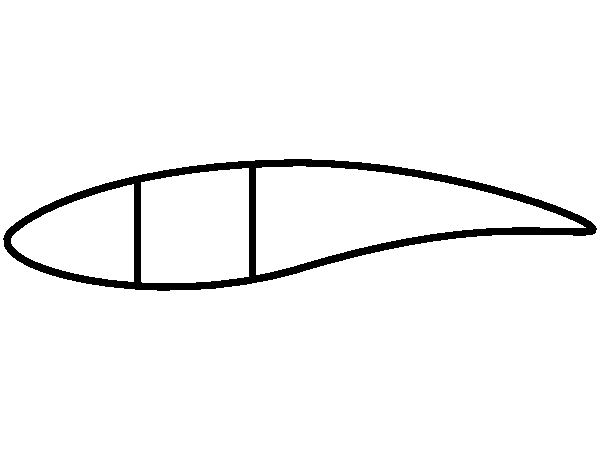
\includegraphics[width=1in]{hollowcore}} &  \parbox[c]{1in}{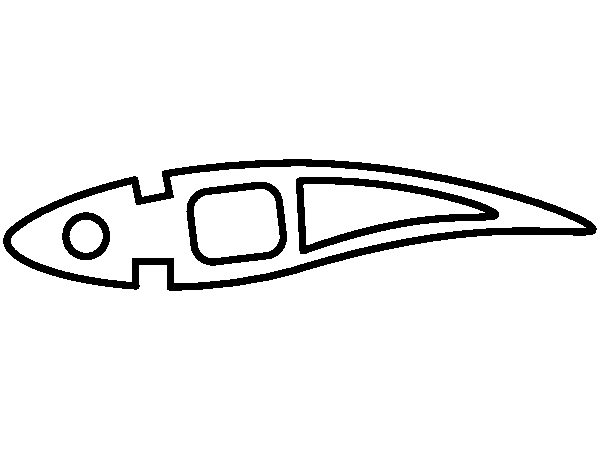
\includegraphics[width=1in]{balsa}} \\
		Weight & 10 & & & \\

		Strength & 8 & & & \\

		Simplicity & 6 & & & \\

		Durability & 4 & & & \\

		{\color{\BYUred} {\color{BYUred} [YEAR SPECIFIC ITEM]}} & 2 & & & \\

		\multicolumn{2}{c }{Totals} &  &  &  \\%BOLD WINNING OPTION

	\end{tabular}
\end{table}

\lipsum[1]


\subsubsection{Empennage Manufacturing Process Selection}

%----------------
%---   Tail Manufacture Decision Matrix  (single prop, dual prop, distributed propulsion, etc.)
%----------------
\begin{table}[h!]
	\centering
	\caption{Weighted decision matrix for tail manufacturing technique.}
	\label{tab:tailmanufacturedecision}
	\rowcolors{2}{white}{BYUbluelite}
\begin{tabular}{ c c c c c } 

	\rowcolor{BYUbluemid}
	& & Foam Core FRP & Hollow Core FRP & Built-up/Balsa \\
	\rowcolor{BYUbluemid}
	Factor & Scale &
	\parbox[c]{1in}{\includegraphics[width=1in]{foamcore}} & \parbox[c]{1in}{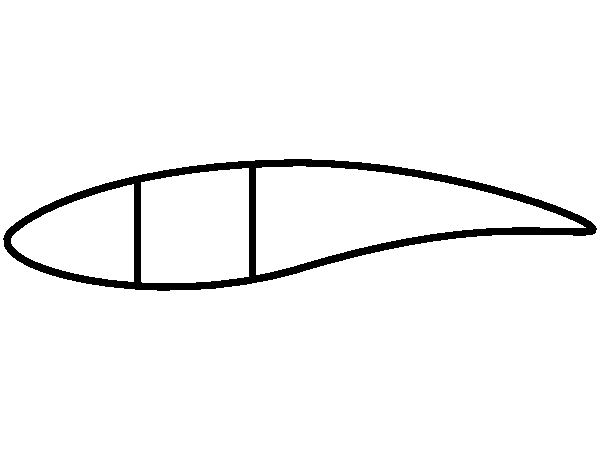
\includegraphics[width=1in]{hollowcore}} &  \parbox[c]{1in}{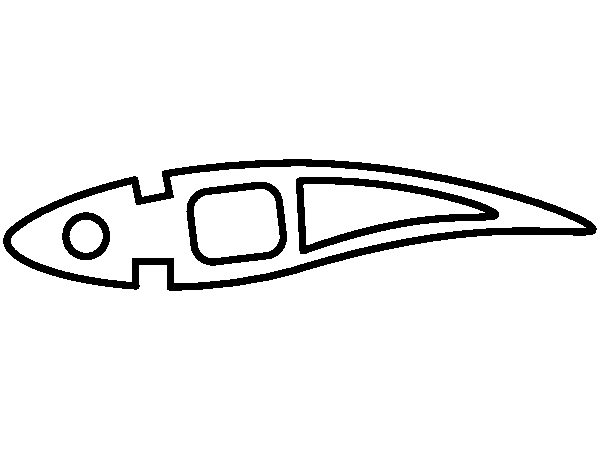
\includegraphics[width=1in]{balsa}} \\

	Weight & 10 & & & \\

	Strength & 8 & & & \\

	Simplicity & 6 & & & \\

	Durability & 4 & & & \\

	{\color{\BYUred} {\color{BYUred} [YEAR SPECIFIC ITEM]}} & 2 & & & \\

	\multicolumn{2}{c }{Totals} &  &  &  \\%BOLD WINNING OPTION

\end{tabular}
\end{table}

\lipsum[1]


\subsubsection{Fuselage Manufacturing Process Selection}

%----------------
%---   Fuselage Manufacture Decision Matrix  (single prop, dual prop, distributed propulsion, etc.)
%----------------
\begin{table}[h!]
	\centering
	\caption{Weighted decision matrix for fuselage manufacturing technique.}
	\label{tab:fuselagemanufacturingdecision}
	\rowcolors{2}{white}{BYUbluelite}
	\begin{tabular}{ c c c c c } 

		\rowcolor{BYUbluemid}
		& & 3D Printing & Hollow Core FRP & Built-up/Balsa \\
		\rowcolor{BYUbluemid}
		Factor & Scale & \parbox[c]{1in}{
\includegraphics[width=1in]{3dprint}} & \parbox[c]{1in}{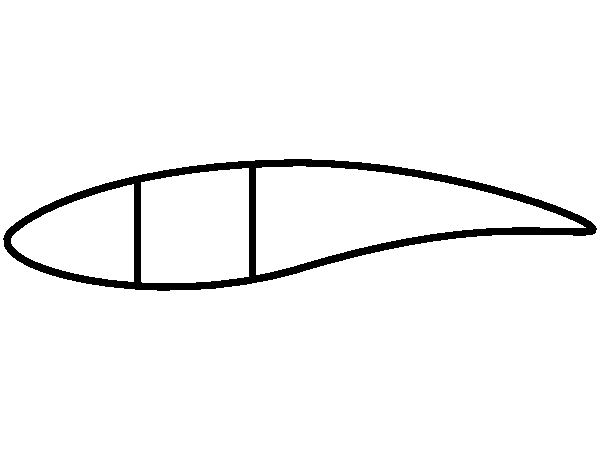
\includegraphics[width=1in]{hollowcore}} &  \parbox[c]{1in}{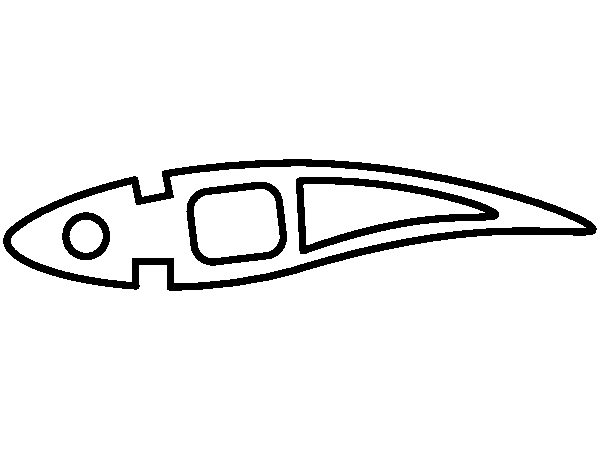
\includegraphics[width=1in]{balsa}} \\

		Weight & 10 & & &\\

		Strength & 8 & & & \\

		Simplicity & 6 & & & \\

		Durability & 4 & & & \\

		{\color{\BYUred} {\color{BYUred} [YEAR SPECIFIC ITEM]}} & 2 & & & \\

		\multicolumn{2}{c }{Totals} &  &  &  \\%BOLD WINNING OPTION

	\end{tabular}
\end{table}

\lipsum[1]



\subsubsection{Payload Manufacturing Process Selection}


%----------------
%---   Payload Manufacture Decision Matrix  (single prop, dual prop, distributed propulsion, etc.)
%----------------
\begin{table}[h!]
	\centering
	\caption{Weighted decision matrix for {\color{\BYUred} [SPECIFY THIS YEAR'S PAYLOAD DESIGN]}.}
	\label{tab:payloadmanufacturedecision}
	\rowcolors{2}{white}{BYUbluelite}
	\begin{tabular}{ c c c c c } 

		\rowcolor{BYUbluemid}
		& & {\color{BYUred} [OPTION]} & {\color{BYUred} [OPTION]} & {\color{BYUred} [OPTION]} \\
		\rowcolor{BYUbluemid}
		Factor & Scale & \parbox[c]{1in}{\includegraphics[width=1in]{draft4x3}} & \parbox[c]{1in}{\includegraphics[width=1in]{draft4x3}} &  \parbox[c]{1in}{\includegraphics[width=1in]{draft4x3}} \\

		Weight & 10 & & &\\

		Strength & 8 & & & \\

		Simplicity & 6 & & & \\

		Durability & 4 & & & \\

		{\color{\BYUred} {\color{BYUred} [YEAR SPECIFIC ITEM]}} & 2 & & & \\

		\multicolumn{2}{c }{Totals} &  &  &  \\%BOLD WINNING OPTION

	\end{tabular}
\end{table}

\lipsum[1]




\subsection{Manufacturing Milestones}
%----------------
% ---  Manufacturing Milestone chart
%----------------
\begin{figure}[h!]
	\centering
	\includegraphics[width=\textwidth]{compiled_figures/manufacturingchart.pdf}
	\caption{This milestone chart reveals our {\color{\BYUblue}original plan} for major elements of our manufacturing process compared to the {\color{\BYUred}actual timing} of these events for our detailed prototype, we hope to hold to a similar planned schedule for our competition build.}
	\label{fig:plannedvsactualtimingmanufacturing}
\end{figure}